% !TEX root = ../thesis.tex

\chapter{Analytical part} \label{sec:analytical}

\section{Introduction} \label{sec:introduction}
Each e-commerce project solves how to predict behavior of their consumers or visitors.
In that complex prediction is usually used statistical methods like a moving average and linear regression in order to
get an idea of consumers behavior.
Basically we need to calculate conversion rate, bounce rate, income value per order and per a customer.
The problem of these values is their non-predictable state by ordinary methods.
Based on Time series analysis we are able to predict
future income but with unsatisfactory aberration.
Better results are produced by trigonometric and polynomial functions as a prediction model.
However on these methods are not applicable psychology and sociology aspects.
There are several statistical methods that can be used to predict income.
In some cases, the reality of the product life cycle is different.
Such irrelevant data therefore complicate management's decisions on the predictive cash flow model of their business.
So let us create better solutions for complex models to predict company income with minimal aberration.
The best approach is to create business plans with that modeling before, so we can minimize the risk of our business.
There are  two phenomena of particular interest in assessing modelling options,  the decoy effect~\ref{subsec:decoy} and vendor lock-in~\ref{subsec:lock-in} principles.
As is written in Models of Consumer Behaviour~\cite{patel}, this modelling is especially used when the new brand or product is established.
Let's teach e-commerce business how to use them on a daily basis and how to overcome the obstacle like a research price for that studies.\\
\\
\textbf{Decoy effect} \label{subsec:decoy}\\
The Decoy Effect or the Asymmetric Dominance Effect is a cognitive bias in which consumers will tend to have a specific
change in preferences between two vendor options when also presented with a third option that is asymmetrically dominated.
Simply put when there is a third strategically important choice, like the decoy, then the consumer is more likely to choose
the more expensive of the other two options.
An option is asymmetrically dominated when it is inferior in all respects to another one.
However, in comparison to the other option, it is inferior in some respects and superior in others.
In other words, it is completely dominated by one option and only partially dominated by the other.
When the asymmetrically dominated option is present, a higher
percentage of consumers will prefer the dominating option like when the asymmetrically dominated option is absent.
The asymmetrically dominated option is therefore a decoy serving to increase preference for the dominating option.\\
\\
\textbf{Lock-in} \label{subsec:lock-in}\\
Proprietary lock-in, or consumer lock, makes the consumer dependent on the products and services of a particular entity
by creating significant costs of switching to the products and services of others.
This can be achieved, for example,
by the use of non-standardized patented product components.
Locking that creates barriers to market entry, can be avoided by antitrust measures.
Proprietary locking is for example blocking mobile phones for only one of the operators or DRM.
\\
\section{Modeling of Human Behavior} \label{sec:modeling}
Overview of mathematical equations and approaches used to modeling in context of Marketing approaches usually used to simulate consumer behavior.
\subsection{Dynamic Model} \label{subsec:dynamicModel}\\
One of the simplest models that have been considered for human behavior modeling are \textbf{dynamic single} prices~\cite{pantland}:

\begin{equation} \label{eq:1}
X_k = f(X_k, t) + \xi(t),
\end{equation}
\\
where the function $f$ is dynamic evolution of vector with possible states $X_k$ at time $k$. $\xi$ is white noise process having known spectral density matrix.
Then we can define an observation process like~\cite{pantland}:

\begin{equation} \label{eq:2}
Y_k = h(X_k, t) + \eta(t),
\end{equation}
\\
where the sensor observation $Y$ is a function of $h$ of the state vector and time. $\eta$ is white noise process having known spectral density matrix.\\
\\
Subsequently, using Kalman results we are able to find the optimal linear estimate as you can see in equation~\ref{eq:3}.\\
\\
The consumer behavior is usually not as simple as a single dynamic model.
For complex model of human behavior we can use some alternatives.
In many cases we have to use different models for each dynamic response of person~\cite{wilsky}.
Afterwards we can test each instance of response to predict a person's state.
From that we can establish \textbf{multiple model} approach to predict future values of state variables.
In these situations is Kalman’s filter calculation very useful for realtime application because of it’s sufficiently small costs of resources.
This approach devide the person’s overall behavior down into several prototypical behaviors~\cite{pantland}.
Mathematically, this is accomplished by setting up a set of states $S$, each associated with a Kalman’s filter and a particular dynamic model.\\
\\
In many situations \textbf{linear ODE model} is used.
In this model the strength of flux between brands and products are determined by perceived brand quality, based upon binary.
The simplest response to such comparisons is an attempt by customers to minimize the expected regret resulting from any choice, which is assumed here.
It has been previously shown that the choice rule recognizes the attribute-wise proximity of an alternative to other brands.
Therefore is appropriate for preference change to be modelled on the pair-wise ranking of brands in each quality.
Probably the easiest way is to assign a positive score to a brand for each successful comparison.
Thus customers attempt to minimize their anticipated regret by opting on any particular quality for a safe bet.
More sophisticated customer behavior, capable of not only ranking brands but discriminating according to the size of proximity gap requires more complex modelling.
However, this may be justified because, at the very least, subjective attribute valuations appear to be non-linear reference point dependent functions.
The ith measurement of innovations process is, intuitively, the part of the observation data that is unexplained by the ith model.
The model that explains the largest portion of the observations is, of course, the model most likely to be correct.
\\
\subsection{Discrete-time model} \label{subsec:discrete}\\
Discrete models or difference equations \footnote{Difference equations can be viewed either as a discrete analogue of differential equations, or independently.
They are used for approximation of differential operators, for solving mathematical problems with recurrences, for building various discrete
models, etc.} are used to describe biological events or whole systems for which is natural to regret time at fixed discrete intervals~\cite{pantland}:

\begin{equation} \label{eq:3}
\hat{X}_{k}^{(i)} = X_{k}^{*(i)} + K_k^{(i)}(Y_k - h^{(i)}(X_{k}^{*(i)},t)),
\end{equation}
\\
where the superscript $(i)$ denotes the $i$th Kalman's filter.
As input $K_k$ Kalman's gain matrix is used for time step $k$.
Then sensor observator $Y$ from equation~\ref{eq:2} is used in combination with $X_{k}^{*}$ as a state prediction matrix.
The measurement innovations process for the $i$th model.\\
\\
The $i$th measurement innovations process is, intuitively, the part of the observation data that is unexplained by the $i$th model.
The model that explains the largest portion of the observations is, of course, the model most likely to be correct.\\
\subsection{Regression model} \label{sec:regression}
A regression model is used to investigate the relationship between two or more variables and estimate one variable based on the others.
In regression analysis, variables can be independent, which are used as the predictor or causal input and dependent, which are used as response variables.


\subsubsection{Linear regression} \label{sec:linear}
As it saw at Linear regression~\cite{linear} linear regression attempts to model the relationship between two variables by fitting a linear equation to observed data.
One variable is considered to be an explanatory variable, and the other is considered to be a dependent variable.
For example, we want to relate the weights of individuals to their heights using a linear regression model.
Before attempting to fit a linear model to observed data, we should first determine if exist a relationship between the variables of interest.
This does not necessarily mean that one variable causes the other, but that there is some significant association between them.
To determine the strength of relationship a scatterplot can be a helpful tool.
If there appears to be no association between the proposed explanatory and dependent variables, then fitting a linear regression
model to the data probably will not provide a useful model.
A valuable numerical measure of association between two variables is the correlation coefficient.
That is a value from $<-1, 1>$ range indicates the strength of the association of the observed data for the two variables.\\
A linear regression line has an equation of the form $Y = a + bX$, where $X$ is the explanatory variable and $Y$ is the dependent variable.
The slope of the line is $b$, and $a$ is the intercept.
Example of some basic linear models:\\
\begin{equation} \label{eq:4}
\begin{array}{l@{}l}
	Y = ax + b\\
	Y = a + bx + c\\
	Y = a\sin x + b\\
\end{array}
\end{equation}

\subsubsection{Polynomial regression} \label{sec:poly}
Polynomial models are a great tool for determining which input factors drive responses and in what direction~\cite{poly}.
These are also the most common models used for analysis of designed experiments.
A quadratic (second-order) polynomial model for two explanatory variables has the form of the equation below.
The polynomial models can be used in those situations where the relationship between study and explanatory variables is curvilinear.
Sometimes a nonlinear relationship in a small range of explanatory variable can also be modelled by polynomials.
The order of the polynomial model is kept as low as possible.
Some transformations can be used for remaining the model to be the first order.
If this is not satisfactory, then the second-order polynomial is tried.
A good strategy should be used to choose the order of an approximate polynomial.
One possible approach is to successively fit the models in increasing order and test the significance of regression coefficients at each step of model fitting.
Another approach is to fit the appropriate highest order model and then delete terms one at a time starting with the highest order.
This continues until the highest order remaining term has a significant statistic.
This is called a backward elimination procedure.
The forward selection and backward elimination procedures do not necessarily lead to the same model.
The first and second-order polynomials are mostly used in practice.
Keep the order increasing until test for the highest order term is nonsignificant.
This is called a forward selection procedure.
Arbitrary fitting of higher-order polynomials can be a serious abuse of regression analysis.
A model which is consistent with the knowledge of data and its environment should be taken into account.
It is always possible for a polynomial of order to pass through n points so that a polynomial of sufficiently high degree can always be found that provides a good fit to the data.
Such models neither enhance the understanding of the unknown function nor be a good predictor.
Example of some basic polynomial models from degree 2 to degree 4:\\
\begin{equation} \label{eq:5}
\begin{array}{l@{}l}
	Y = ax^2 + b\\
	Y = ax^2 + bx + c\\
	Y = ax^3 + bx^2 + cx + d\\
	Y = ax^4 + bx^3 + cx^2 + dx + e\\
\end{array}
\end{equation}

\section{Prediction of Human Behavior} \label{sec:prediction}
Overview of mathematical approaches used to predict consumer behavior.
Based on equation~\ref{eq:3},\ we can continue to find optimal linear estimate $X_k$ using the Kalman's filter~\cite{pantland}: \footnote{In statistics
and control theory, Kalman filtering, also known as linear quadratic estimation (LQE), is an algorithm that
uses a series of measurements observed over time, containing statistical noise and other inaccuracies, and produces
estimates of unknown variables that tend to be more accurate than those based on a single measurement alone, by estimating
a joint probability distribution over the variables for each timeframe.
The filter is named after Rudolf E. Kálmán, one of the primary developers of its theory.}

\begin{equation} \label{eq:6}
X = X_{k}^{*} + K_x(Y_k - h(X_{k}^{*},t)),
\end{equation}
\\
provided that the Kalman gain matrix $K_k$ is chosen correctly~\cite{kalman}.
This method iterates for each step $k$ and the filter algorithm use a state prediction at each time step $k$, the filter algorithm
uses a state prediction $X$, an error covariance matrix prediction $P_k^*$, and a sensor measurement $Y_k$ to determine an optimal linear state estimate $X$.
If we want to predict human’s future state, we can use this mechanism with larger time steps.
This mechanism is used e.g. in a car, where such a prediction capability can allow us to maintain synchrony with the driver.
In experience of Alex Pentland work \footnote{MIT's Human Dynamics Laboratory and the MIT Media Lab Entrepreneurship
Program, co-leads the World Economic Forum Big Data and Personal Data initiatives, and is a founding member
of the Advisory Boards for Nissan, Motorola Mobility, Telefonica, and a variety of start-up firms.} this type of prediction is useful only for short time periods,
for instance, in the case of quick hand motions for up to one-tenth of a
Especially $f$, $h$ are linear functions and $\xi$, $\eta$ are gaussian.
These functions are commonly extended to "well-behaved" nonlinear problems by approximating
the nonlinear system by linear functions using a local Taylor expansion\footnote{Taylor series is a representation of a function
as an infinite sum of terms that are calculated from the values of the function's derivatives at a single point.}.

\subsection{Specification of customer behavior} \label{subsec:specification}
Products for customers such as shampoo or tomato sauce are designed to appeal to customers and encouraging them to buy those products.
It depends on the industry section but all of that designs try to focus on customer’s subconscious.
However, buying behavior is not only a function of the product.
In many cases is the connection of many other functions like a social environment of other customers, the competing products in the marketplace,
brand marketing strategy, seller trust and professionalism and so on.
In order to design the best product, it is inevitable to understand not only the physics and chemistry of the product,
but also the psychology of customers and the sociology of customer groups or networks\cite{patel}.
From that paragraphs is obvious that the general customer behavior model has many input variables to represent many
kinds of situations to be successfully in future prediction.
A good model in the business industry must be able to learn from the actual behavior of the customer at each seller and learn from these data sets in a macroscopically averaged way.
Alternatively, we can look at individual customers and their shopping behavior and try to derive large-scale observable effects.
Ideally we can predict behavior for each customer and from these results we are able to create a global results for each store or industry.\\
\\
\textbf{Loyalty} \label{subsec:loyalty}\\
Loyalty is the tendency for some customers to use the same products or brands again.
This behavior we can describe with systems of ordinary differential equations.
The stronger the loyalty, the slower the changes in the number of people buying specific products.
For discrete-time models, the degree of loyalty corresponds to the size of diagonal elements in a transition matrix.
During the modelling we have to calculate with  disloyalty model too.
In some industries like a supermarkets,
people buy from other reason, so some of our input variables in modelling should be detection of loyalty in out industry.
Next aspect of loyalty could be a memory effect which represent people returning to products they had previously used,
after trying something new they then did not like.
This could be taken into account perhaps by using recurrence
relations or differential equations of higher than first order or even employing delay-differential equations.\\
\\
\textbf{Sociology} \label{subsec:sociology}\\
In this context, we can understand sociology as a process where people influence other people with their purchases.
In nowadays there is some kind of trend when people buy same brands or products.
As was mentioned in part lock-in~\ref{subsec:lock-in},
there exist an option with one product dominating the market.
This possibility is very hard to test in relevant way, because data of big  companies which dominates in some kind of industry are very hard to get legally.
Even if their competitors have more or less identical products.
This effect and its opposite, are easily modelled by discrete-time models (see section ~\ref{subsec:discrete}).
Opposite is very important in sociology because of people wanting to be different sometimes from irrationals reasons.

\subsection{Markov Chains} \label{subsec:chain}
A Markov chain is a process that occurs in a series of time-steps.
In each is a random choice is made among a finite (or also enumerable) number of states since both  the index set and
the state space are discrete, as is seen on figure~\ref{markovmodel}, then we denote by~\cite{patel}:\\
\begin{equation} \label{eq:7}
\begin{array}{l@{}l}
	p_{ij}=P[X_{n+1}=j|X_n=i],
\end{array}
\end{equation}\\
where $p_{ij}$ is the probability of moving from state $i$ to state $j$, then the transition probability is represented by a matrix.\\
For homogeneous chains, these probabilities do not depend on $n$, i.e., they are stationary.
Then, the initial distribution, together with the transition matrix P, determines the probability distribution for any state at all future times.\\
\begin{figure}[h!]
	\begin{center}
		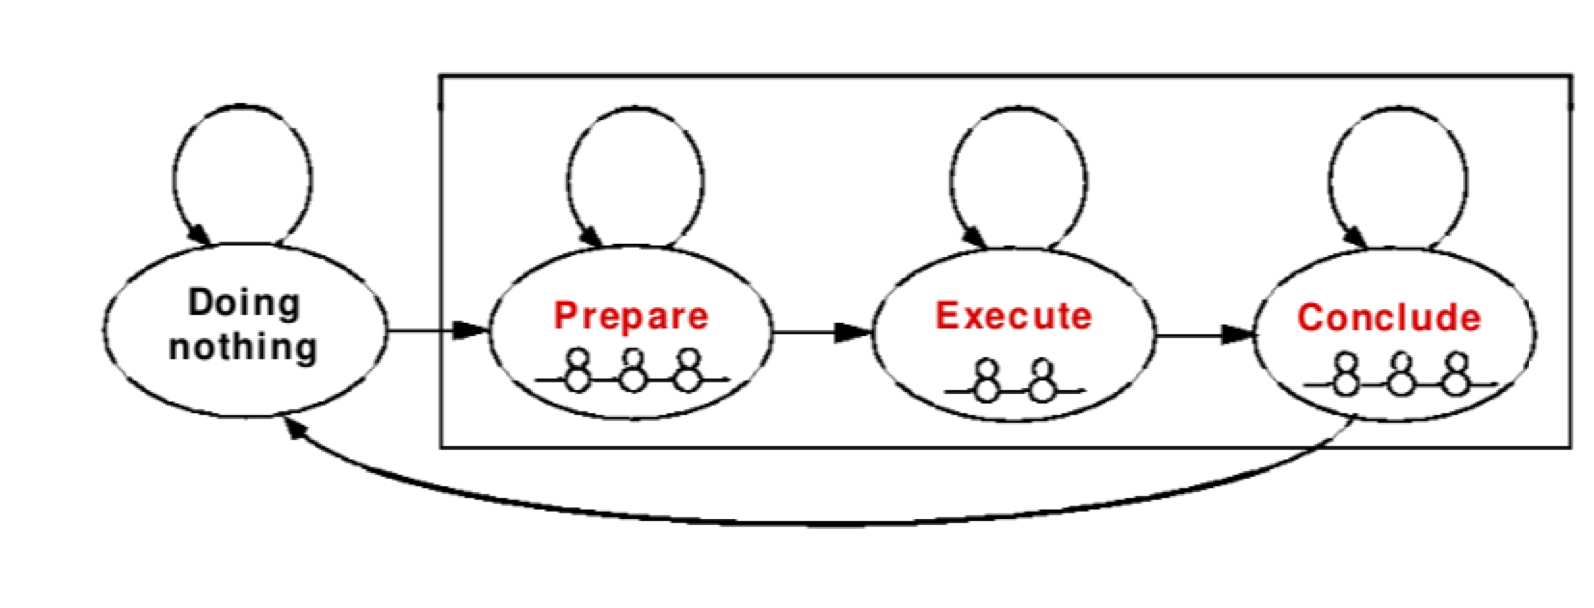
\includegraphics[width=120mm]{markov_model.png}
	\end{center}
	\caption{Basic schema of Markov model in human decision~\cite{patel}}
	\label{markovmodel}
\end{figure}\\
\textbf{Hidden Markov model} \label{subsec:hmm}\\
The statistical implementation of Markov chain in which the system being modeled is assumed to be a Markov process $X$ with unobservable states.
HMM assumes that there is another process $Y$ with dependent behavior on $X$.
This approach is used to learn about $X$ by observing $Y$.
The states of the process $X_n$ are hidden states and the result from equation:\\
\begin{equation} \label{eq:8}
P = (Y_n ∈ A|X_n = x_n),
\end{equation}\\
where $P$ is emission probability (some time called output probability) and $X_n$ is Markov process which is not directly observable.
Both $Y_n$ and $X_n$ let it be discrete-time processes.
For every $n \geg 1, x_1,\ldots ,x_n$ and an arbitrary (measurable) set $A$.\\
This method is without any memory so past doesn't mather, only future is important and relevant for HMM.\\
\\
\textbf{A Markov model with social influences} \label{subsec:markov}\\
This model is based on Markov chains, an stochastic model describing a sequence of possible events in which the probability
of each event depends only on the state attained in the previous event.
A countably infinite sequence, in which the chain moves
state at discrete time steps, gives a discrete-time Markov chain (DTMC).
A continuous-time process is called a continuous-time Markov chain (CTMC).
It is named after the Russian mathematician Andrey Markov.
This method is actually better for our purpose than the time continues differential equations which are usually used for prediction.
In order to use this model approach, first of all we have to develop the possibility of a decoy effect.
Then we introduce sociology and obtain results for lock-in analogous.
These Markov models display both important similarities to and differences from the previous models, and may be simpler to work with.
The last but not the least pros of that models is very good graphical representation.\\
\\
\textbf{An Experiment Using Markov Dynamic Models} \label{subsec:markov_dynamic}\\
Shopping is natural-feeling and familiar type of human behavior that exhibits complex patterns that last from several seconds to several days.
These characteristics make shopping almost ideal experimental for modeling human behavior.
In the case of shopping, the macroscopic actions are events like needs, choosing brands, choosing seller.
The internal states are the individual steps that make up the action, and the observed variables will be changes during the shopping
process workflow in which can be decision of customer different.
The intuition is occasionally important, but this belongs to special market and marketing personal identification such a buying shoes by a single woman in production age.\\
\\
\textbf{Modeling and Prediction of Human Behavior may consist of the following steps:}\\
\begin{enumerate}
	\item needs decision make
	\item looking across the site to find some adequate
	\item make action decision
	\item shopping workflow process in selected site
	\item make final payment
\end{enumerate}
\\
In this case psychology covers how and what influence people to make thier choises of actual items on the shelves in
shop and the possible reason why they will buy something different from previously.
Advertising might be comprised into these characteristics but could also possibly be considered as part of the sociological
influences (point 1 and 2), especially if the advertising takes the form of a well known figure endorsing a product.
More specifically, the following four properties have been identified by Unilever Research~\cite{patel} as being important and their influence were included in one or more models:

\begin{enumerate}
	\item Regret.
	This refers just two products compare with each other as regards different qualities, which can include price (or its inverse value).
	A customer might judge one item to be superior to another in all respects.
	\item Attribute change.
	The introduction of a new product onto the market can change the way of customers, or at least some of them, view established brands.
	This might be by drawing attention to some quality which was not previously much regarded, or it might make people give different
	weightings to the (established) qualities when making their decisions. The former can be considered to be a special case of the latter.
	\item Outlier avoidance.
	When a number of products are in many aspects quite similar, there can be a tendency for people to avoid ‘strange’ ones,
	like others which are substantially different from the majority in price or some other respect.
	Items near the average can be favoured.
	\item Decision process change.
	Decision process change.
	A straight choice between two items might be relatively easy.
	They can be compared according to price, size etc\. and a decision made. With three or more,
	comparisons might be made between two things at a time, one could be eliminated and then the winner contrasted with a third.
\end{enumerate}
\subsection{Viterbi algorithm} \label{subsec:viterbi}
The Viterbi algorithm is a dynamic programming algorithm for finding the most likely sequence of hidden states called
the Viterbi path that results in a sequence of observed events, especially in the context of Markov information
sources and hidden Markov models (HMM).\\
The algorithm has found universal application in decoding the convolutional codes used in both CDMA and GSM digital cellular,
dial-up modems, satellite, deep-space communications, and 802.11 wireless LANs.
Now it is also commonly used in speech recognition, speech synthesis, keyword spotting, computational linguistics, and bioinformatics.
For example, in speech-to-text (speech recogni- tion), the acoustic signal is treated as the observed sequence of events, and a string of text is considered
to be the "hidden cause" of the acoustic signal.
The Viterbi algorithm finds the most likely string of text given the acoustic signal~\cite{DBLP:journals/corr/abs-cs-0504020}. \\

\subsection{Predicted effects} \label{subsec:predicted}
\begin{enumerate}
	\item How a decoy product might influence the market.
	The appearance of a third product might remarkably change the market shares of two others, while getting minimal sales itself.
	This effect is one of the most complex biases in customer choice, and has been observed in product classes from chocolate bars to electronics to beer.
	The decoy effect illustrates the importance of customer psychology, to understand how customers recognize products, and how customers see quality side to buy the product.

	\item The dynamics of market share is how sales of products can change during the time.
	For example, even if two products are really equal in all relevant aspects, then after a long time of customer
	activity it might be that each product takes 50\% market share (preserving the symmetry), or one product takes
	nearly 100\% market share (breaking the symmetry), or that there is no steady state, with market dominance alternating between the two brands.
	The second of these three cases is called lock-in, corresponding to one brand obtaining a virtual monopoly, which is almost impossible to break.
	From that reason is not legally to create a monopole in some industries and for human purchase behavior is not good to calculate with monopole approach.

	\item How a new product will fare, given its quality profile compared with existing brands.
	This question is complementary to that of the decoy, asking what market share a new product will gain rather than how it will affect the market shares of existing products.

	\item A choice overload: when there are too many possible options for potential customers from which they can pick,
	many of them will search the sites without making a
	\item Minimise anticipated regret modelling property was taken to lead to simple comparisons along the lines of with regard to quality $k$,
	is product $i$ better than product $j$?
	If the answer to all relevant questions, $k = 1, . . . , nq$, if $nq$ is the number of qualities, is no, then a customer
	will not change from $j$ to $i$.
	The more times the answer is yes, the faster such a change is likely to happen.
\end{enumerate}
\\
\section{Customer preferences and decision process} \label{sec:customer_preferences}
Considering a customer whose preference is shared out amongst all the available brands in a market where there are no empty or zero brands,
so that the total of all brands preference shares is 1 (100\%).
The proportion of customer preference held by brand $X$ at time $t$ is denoted by $X(t)$.
For example, if the preference share of brand A is plotted against brand B in a market where only two brands exists,
the point must be somewhere along the straight line $B(t) = 1, A(t)$.
Of interest is the case when a third brand is added, possibly as a
The additional brand means that the preference distribution changes from being a straight line in the two-dimensional plane $(A, B)$,
to a plane in three-dimensional space $(A, B, C)$.\\
\\
\textbf{Customer decision process} \label{sec:cus_decision} described in~\cite{patel} show that the standard Logit model~\ref{subsec:logit} for customer choice assumes that
the probability, $p_i$, with which a customer buys a given product $i$ from a range of products $<1, n>$ depends on
the value which customer internally assigned to that product and his price.
This dependence is taken to be of exponential form.
Assuming that guaranteeing that all probabilities are positive)
\\
\begin{equation} \label{eq:9}
p_i = C\exp(V_i - sP_i),
\end{equation}
\\
where $s$ is a measure of the relative importance of price to the customer, and $C$ is a normalisation constant set to be results always positive. $V_i$ is subjective value
attached to product by a customer with dependency on price of the product $P_i$.~\cite{patel}:
\\
\begin{equation} \label{eq:10}
\sum_{i=1}^n p_i = 1.
\end{equation}
\\
The value $V_i$ is then taken to reflect the influence on the customer of the quality of the product,$Q_i$,
the increased likelihood of the customer buying the same brand as he bought previously (the loyalty effect),
and the peoples who have an influence on a customer (neighbours).
Each of these dependencies are taken to be linear, giving~\cite{patel}:
\\
\begin{equation} \label{eq:11}
V_i = aQ_i + lI_i + hN_i,
\end{equation}
\\
where $I_i$ is an indicator function which is unity if the customer a previously bought product i and zero otherwise,
$N_i$ is the number of neighbours who bought product $i$, and $a, l$ and $h$ are constants measuring the relative strength
of each effect.
In such a model the products are all treated independently.
Only coupling between the probabilities occurs through the normalisation constant $C$.
Product $I$ will depend not only on the value and price of that product, $V_i$ and $P_i$, but on the value and prices of all products.
The goal of this section is to formulate a model for this probability which is based on binary comparisons, that is,
on comparisons of two products at a time.\\
\subsection{Logit analysis in marketing} \label{subsec:logit}
Logit analysis is a statistical technique used by marketers to assess the scope of customer acceptance of a product, particularly a new product.
It attempts to determine the intensity or magnitude of customers' purchase intentions and translates that into a measure of actual buying behavior.
Logit analysis assumes that an unmet need in the marketplace has already been detected, and that the product has been designed to meet that need.
The purpose of logit analysis is to quantify the potential sales of that product.
It takes survey data on consumers purchase intentions and converts it into actual purchase probabilities.
Logit analysis defines the functional relationship between stated purchase intentions and preferences, and the actual probability of purchase.
A preference regression is performed on the survey data.
This is then modified with actual historical observations of purchase behavior.
The resultant functional relationship defines purchase probability.

\subsection{Brand or product changing} \label{subsec:brand}
We can mathematically express the process of decision to switch from one brand to another one.
Consider a linear flux $\alpha_{xy}$ of preferences moving to brand $X$ from brand $Y$.
All fluxes have to be strictly positive.
It's in improper to consider negative flux, so really excluded is only zero value.
Flux is the proportion of customer preference to switch to other brand or product from previous one.
\begin{figure}[h!]
	\begin{center}
		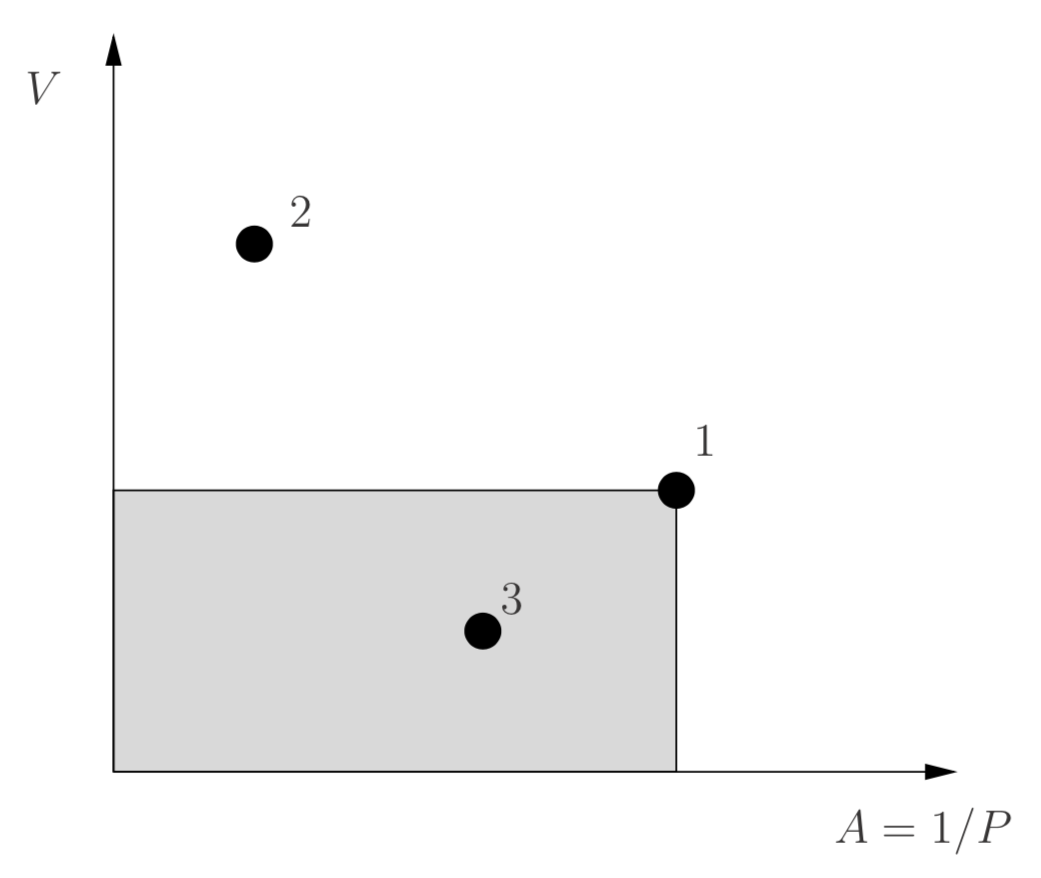
\includegraphics[width=80mm]{affordability.png}
	\end{center}
	\caption{Products in the affordability-value plane.
	The shaded region is the region of products dominated by product 1~\cite{pantland}.}
	\label{Affordability of products}
\end{figure}
\\
The basic idea from Models of Consumer Behaviour~\cite{patel} is to build a model based on a physical analogy,
between the customers buying behavior and particle-particle dynamics.
Let us assume customers to be particles moving in quality space.\\
\begin{figure}[h!]
	\begin{center}
		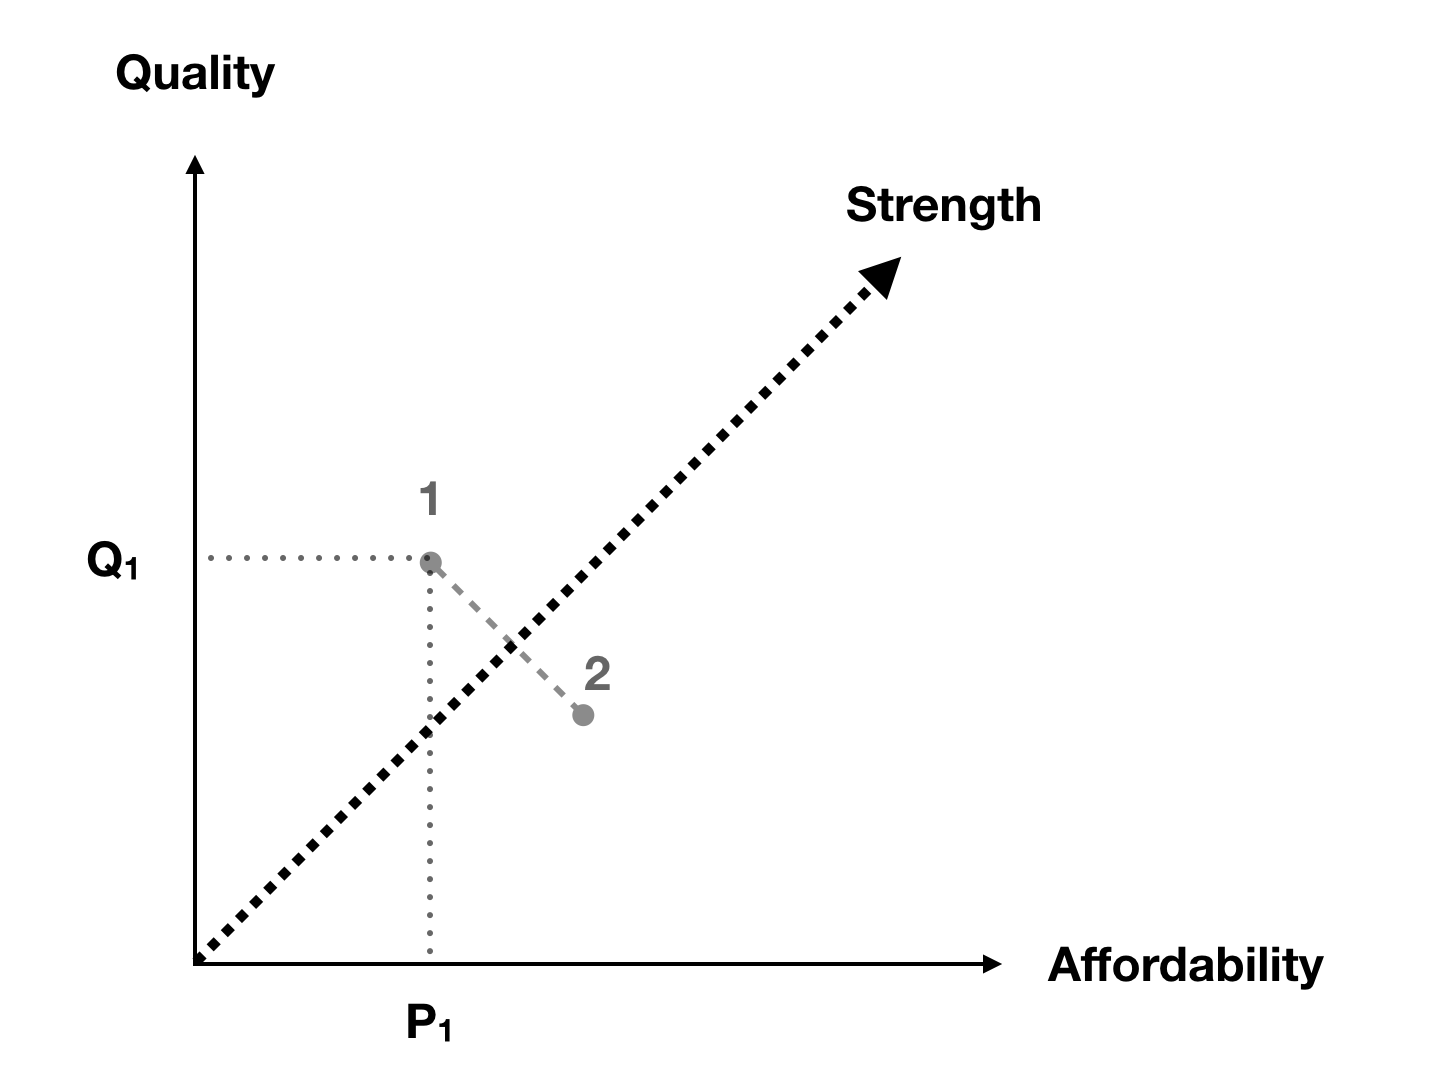
\includegraphics[width=80mm]{strength.png}
	\end{center}
	\caption{Product space with two products~\cite{patel}}
	\label{Strength of products}
\end{figure}
\\
The products are considered as sources of  potentials strength, the details of the potentials depending on the products’ characteristics.
The psychology of people will be regarded as the influence of the potential on the mass of the particles.
This will depend on the customer but also on the characteristics of each product, weighted by coefficients of choice.
The sociology of individuals can be considered as a form of particle-particle interaction. Following what has gone before,
the product space is defined by just two characteristics for each product $i$ with affordability $P_i$ and quality $Q_i$.
We can define the ‘strength’\footnote{The power if the product or service to be attractive for customer.} of a product as
the distance of the product from the origin in product space as~\cite{pantland}:
\\
\begin{equation} \label{eq:12}
U_i = \frac{(P_i + Q_i)}{2}.
\end{equation}
\\
All the products with $P_i + Q_i = constant$ will have the same strength.
